\documentclass{standalone}
\usepackage{tikz}
\usepackage{xinttools}

\usetikzlibrary{calc,math}


\newcommand{\cliphalfplane}[2]{
  \ifnum#1=#2
  \else
    \path[clip] ($ (P#1) ! {sin(45)} ! 45:(P#2) $) -- ($ (P#1) ! {sin(45)} ! -45:(P#2) $) -- ([turn]0:\dist) -- ([turn]-90:2*\dist) -- ([turn]-90:4*\dist) -- ([turn]-90:2*\dist) -- cycle;
  \fi
}

\newcommand{\drawarea}[2]{
  \begin{scope}
    \xintFor ##1 in {1,2,3,4,5,6} \do {
      \cliphalfplane{#1}{##1}
    }

    \draw[fill=#2] (-3,-3) rectangle (3,3);
  \end{scope}
}


\begin{document}

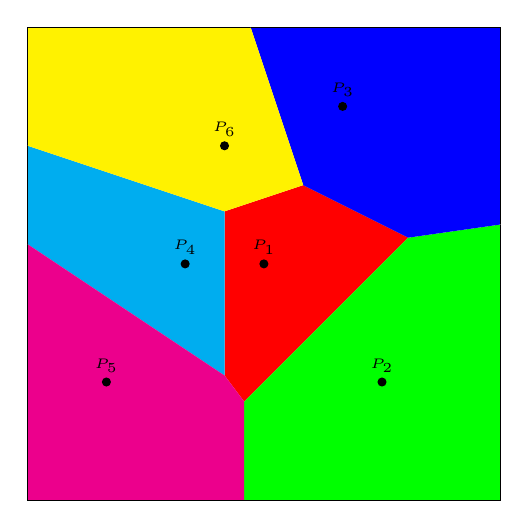
\begin{tikzpicture}
  \tikzmath{
    real \dist;
    \dist = 5;
  }
  \path[use as bounding box] (-3,-3) rectangle (3,3);
  \coordinate (P1) at (0,0);
  \coordinate (P2) at (1.5,-1.5);
  \coordinate (P3) at (1,2);
  \coordinate (P4) at (-1,0);
  \coordinate (P5) at (-2,-1.5);
  \coordinate (P6) at (-0.5,1.5);

  \drawarea{1}{red}
  \drawarea{2}{green}
  \drawarea{3}{blue}
  \drawarea{4}{cyan}
  \drawarea{5}{magenta}
  \drawarea{6}{yellow}

  \foreach \i in {1,...,6} {
    \draw[fill=black] (P\i) circle [radius=0.05cm] node[above,font=\tiny] {$P_{\i}$};
  }
\end{tikzpicture}

\end{document}